\subsection{The averaged cube estimate at weak coupling: necessary
conditions, the free field, and the plaquette}\label{rD:sec}

Throughout, $G$, $\varphi$, $\Lambda=\Lambda_L$, $E$, $P$, $\mu$, $V_x$,
$X$, $\mathcal P_x$ and $\mathcal A$ are as in Sec.~\ref{ssec:averaged},
$n\ge2$, so that $X=\Lambda_L$ on the torus, and
\[
\mathcal E_n(f)=\frac1{n^4}\sum_{x\in X}\mu\bigl((f-\mathcal P_xf)^2\bigr)
\]
is the Dirichlet form of Definition~\ref{def:avgcube}, as in
Sec.~\ref{ssec:bpweak}, so that $\mathrm{BP}(n,\varpi)$ reads
$\varpi\Var_\mu(f)\le\mathcal E_n(f)$ for real $f\in\mathcal A$. For
$V\subset E$ let $P(V)$ be the set of plaquettes of $P$ that contain a link
of $V$, and $\mathcal F_V$ the $\sigma$-algebra generated by the links
outside $V$; thus $\mathcal P_x$ is the conditional expectation given
$\mathcal F_{V_x}$. In this subsection $\partial$ denotes the boundary
operator on chains, the transpose of the coboundary $d$ (the set
$\partial V$ of Sec.~\ref{ssec:averaged} is not used). The lattice is the torus
$\Lambda_L=(\Z/L\Z)^4$; coordinates are taken in $\Z/L\Z$, and when
$L\ge n+2$ the residues $x_i-1,x_i,\dots,x_i+n$ are distinct, so that
$x_i-1$ and $x_i+n$ lie outside $x_i+[0,n)$. A plaquette $(y,\mu\nu)$,
$\mu<\nu$, has the links $(y,\mu)$, $(y+e_\mu,\nu)$, $(y+e_\nu,\mu)$,
$(y,\nu)$, with base points $y,y+e_\mu,y+e_\nu,y$, and
$U_p=U_{(y,\mu)}U_{(y+e_\mu,\nu)}U_{(y+e_\nu,\mu)}^{-1}U_{(y,\nu)}^{-1}$.

\subsubsection{The plaquettes read by one cube}

\begin{lemma}[layers]\label{rD:layer}
Let $L\ge n+2$, $x\in\Lambda_L$, let $\{\mu,\nu\}$ be a plane and
$\rho,\sigma$ the two other directions. For $t=(t_\rho,t_\sigma)\in
(x_\rho+[0,n))\times(x_\sigma+[0,n))$ let $Q_t$ be the set of the
$(n+1)^2$ plaquettes $(y,\mu\nu)$ with $y_\rho=t_\rho$, $y_\sigma=t_\sigma$,
$y_\mu\in x_\mu+[-1,n-1]$, $y_\nu\in x_\nu+[-1,n-1]$; let $q_t\in Q_t$ be
the plaquette with $y_\mu=x_\mu-1$, $y_\nu=x_\nu-1$, and $R_t=Q_t\setminus
\{q_t\}$.
\begin{enumerate}[label=\textup{(\roman*)},leftmargin=*]
\item The plaquettes of $P(V_x)$ in the plane $\{\mu,\nu\}$ form the
disjoint union of the $n^2$ sets $R_t$; each has $(n+1)^2-1$ elements. In
particular $\lvert P(V_x)\rvert=6n^2\bigl((n+1)^2-1\bigr)$, and for a fixed
plaquette $p$ the number of $x$ with $p\in P(V_x)$ is $n^2((n+1)^2-1)$,
while the number of $x$ such that all four links of $p$ lie in $V_x$ is
$n^2(n-1)^2$.
\item No link of $q_t$ lies in $V_x$, so $q_t\notin P(V_x)$; every link
$(y,\mu)$ with $y_\nu\in\{x_\nu-1,x_\nu+n\}$ and every link $(y,\nu)$ with
$y_\mu\in\{x_\mu-1,x_\mu+n\}$ lies outside $V_x$. The boundary $1$-chain
$\partial R_t=\partial Q_t-\partial q_t$ is supported on such links and on
the links of $q_t$, hence on links outside $V_x$.
\item If $G$ is abelian, $\prod_{p\in R_t}U_p=\prod_{e}U_e^{(\partial
R_t)_e}$ is a function of the links outside $V_x$, hence
$\mathcal F_{V_x}$-measurable.
\end{enumerate}
\end{lemma}

\begin{proof}
(i) A plaquette $(y,\mu\nu)$ lies in $P(V_x)$ if and only if one of the
base points $y,y+e_\mu,y+e_\nu$ lies in $x+[0,n)^4$. All three have the
transverse coordinates $y_\rho,y_\sigma$, so $y_\rho\in x_\rho+[0,n)$ and
$y_\sigma\in x_\sigma+[0,n)$ are necessary, which gives the $n^2$ values of
$t$. In the plane, with $A=(x_\mu+[0,n))\times(x_\nu+[0,n))$, the condition
is $(y_\mu,y_\nu)\in A\cup(A-e_\mu)\cup(A-e_\nu)$. A point of
$(x_\mu+[-1,n-1])\times(x_\nu+[-1,n-1])$ lies in $A$ if both coordinates
are at least $x_\mu$, resp.\ $x_\nu$; in $A-e_\mu$ if $y_\mu=x_\mu-1$ and
$y_\nu\ge x_\nu$; in $A-e_\nu$ if $y_\nu=x_\nu-1$ and $y_\mu\ge x_\mu$; and
the point $(x_\mu-1,x_\nu-1)$ lies in none of the three. Conversely the
union lies in that square. So the plaquettes of $P(V_x)$ in the plane with
transverse position $t$ are exactly $R_t$, of cardinality $(n+1)^2-1$.
Summing over the six planes gives $\lvert P(V_x)\rvert$. For fixed $p$, the
number of $x$ with $p\in P(V_x)$ equals, by translation, the number of
plaquettes of $P(V_0)$ in the plane of $p$, that is $n^2((n+1)^2-1)$. All
four links of $p=(y,\mu\nu)$ lie in $V_x$ if and only if $y,y+e_\mu,y+e_\nu
\in x+[0,n)^4$, that is $x_\rho,x_\sigma\in y_\rho+(-n,0],y_\sigma+(-n,0]$
($n$ values each) and $x_\mu\in[y_\mu+2-n,y_\mu]$, $x_\nu\in[y_\nu+2-n,
y_\nu]$ ($n-1$ values each), which gives $n^2(n-1)^2$.

(ii) The base point of a link $(y,\mu)$ is $y$; if $y_\nu\in\{x_\nu-1,
x_\nu+n\}$ then $y\notin x+[0,n)^4$ since $L\ge n+2$. The same holds for
$(y,\nu)$ with $y_\mu\in\{x_\mu-1,x_\mu+n\}$. The links of $q_t$ are
$(q_t,\mu)$, $(q_t,\nu)$ with base point $(x_\mu-1,x_\nu-1)$ in the plane,
$(q_t+e_\mu,\nu)$ with base point $(x_\mu,x_\nu-1)$, and $(q_t+e_\nu,\mu)$
with base point $(x_\mu-1,x_\nu)$; each has a coordinate $x_\mu-1$ or
$x_\nu-1$, so none lies in $V_x$. Since $\partial$ is linear and each link
interior to the square $Q_t$ lies in two of its plaquettes with opposite
orientations, $\partial Q_t$ is supported on the links $(y,\mu)$ with
$y_\nu\in\{x_\nu-1,x_\nu+n\}$, $y_\mu\in x_\mu+[-1,n-1]$, and $(y,\nu)$ with
$y_\mu\in\{x_\mu-1,x_\mu+n\}$, $y_\nu\in x_\nu+[-1,n-1]$; and $\partial R_t=
\partial Q_t-\partial q_t$ is supported on these links and those of $q_t$.

(iii) For abelian $G$, $U_p=\prod_eU_e^{(\partial p)_e}$, so $\prod_{p\in
R_t}U_p=\prod_eU_e^{(\partial R_t)_e}$, and by (ii) only links outside
$V_x$ occur.
\end{proof}

\begin{lemma}[walls]\label{rD:walls}
In the setting of Lemma~\ref{rD:layer}, put $s=x_\rho+n-t_\rho\in[1,n]$ and
$Q'_t=Q_t+se_\rho$, the translate of $Q_t$ to the transverse position
$(x_\rho+n,t_\sigma)$. There is an integer $2$-chain $W_t$, supported on
plaquettes of the planes $\{\mu,\rho\}$ and $\{\nu,\rho\}$ that do not lie
in $P(V_x)$, such that $Q'_t\cap P(V_x)=\emptyset$ and such that every real
$2$-cochain $F$ on $\Lambda_L$ with $dF=0$ satisfies
\[
\sum_{p\in R_t}F_p=\sum_{p\in Q'_t}F_p+\ip F{W_t}-F_{q_t}.
\]
If $G$ is abelian and $U_p$ are the plaquette variables of a configuration
$U$, then
\[
\prod_{p\in R_t}U_p=\prod_{p\in Q'_t}U_p\prod_pU_p^{(W_t)_p}U_{q_t}^{-1}.
\]
In both cases the left side is a function of the plaquette variables of
plaquettes outside $P(V_x)$.
\end{lemma}

\begin{proof}
For $z\in\Lambda_L$ let $c(z)$ be the $3$-cell with corner $z$ spanned by
$e_\mu,e_\nu,e_\rho$, oriented so that
\[
\begin{split}
\partial c(z)&=(z+e_\rho,\mu\nu)-(z,\mu\nu)+\bigl[(z,\mu\rho)-(z+e_\nu,\mu
\rho)\bigr]\\
&\quad+\bigl[(z+e_\mu,\nu\rho)-(z,\nu\rho)\bigr]
\end{split}
\]
up to a common sign of the two brackets, which plays no role below. Put
$T=\sum_{j=0}^{s-1}\sum_{z\in Q_t}c(z+je_\rho)$, where $z\in Q_t$ stands for
the corner of the plaquette. In $\partial T$ the $\mu\nu$-faces telescope
in $j$ and give $\sum_{z\in Q_t}\bigl[(z+se_\rho,\mu\nu)-(z,\mu\nu)\bigr]=
1_{Q'_t}-1_{Q_t}$. For fixed $j$ the $\mu\rho$-faces of the cells $c(z+j
e_\rho)$, $z\in Q_t$, are $(z+je_\rho,\mu\rho)$ and $(z+je_\rho+e_\nu,\mu
\rho)$ with opposite signs; as $z_\nu$ runs over $x_\nu+[-1,n-1]$ the faces
with $z_\nu\in x_\nu+[0,n-1]$ cancel against those of the neighbour, and
the survivors have $\nu$-coordinate $x_\nu-1$ or $x_\nu+n$. In the same way
the surviving $\nu\rho$-faces have $\mu$-coordinate $x_\mu-1$ or $x_\mu+n$.
Let $W_t=\partial T-(1_{Q'_t}-1_{Q_t})$ be the chain of these survivors.
A plaquette $(y,\mu\rho)$ has links with base points $y,y+e_\mu,y+e_\rho$,
all with $\nu$-coordinate $y_\nu$; if $y_\nu\in\{x_\nu-1,x_\nu+n\}$ none of
them lies in $x+[0,n)^4$, so the plaquette is not in $P(V_x)$. The same
holds for the $\nu\rho$-faces. A plaquette of $Q'_t$ has all base points
with $\rho$-coordinate $x_\rho+n$, so it is not in $P(V_x)$ either. Since
$L\ge n+2$, the coordinates $x_i-1,\dots,x_i+n$ occurring in $T$ are
distinct residues, so no two cells of $T$ coincide and the cancellations
are as described.

If $dF=0$ then $\ip F{\partial T}=\ip{dF}T=0$, that is $\sum_{Q_t}F_p=
\sum_{Q'_t}F_p+\ip F{W_t}$, and subtracting $F_{q_t}$ gives the first
identity. For abelian $G$ and every $3$-cell $c$, $\prod_pU_p^{(\partial
c)_p}=1$, since each link of $c$ lies in two of its faces with opposite
orientations; hence $\prod_pU_p^{(\partial T)_p}=1$, which is the second
identity after multiplication by $U_{q_t}^{-1}$. Lemma~\ref{rD:layer}(ii)
shows $q_t\notin P(V_x)$.
\end{proof}

\subsubsection{The free Maxwell field: the averaged condition fails at the
diffusive rate}

Let $C^k$ be the real $k$-cochains on $\Lambda_L$ with the $\ell^2$ pairing
$\ip\cdot\cdot$, $d$ the coboundary and $\partial=d^{\mathrm T}$, so that
$d\circ d=0$ and $\ip{dA}S=\ip A{\partial S}$. Let $B=dC^1\subset C^2$ be the
exact $2$-cochains and $\Pi$ the orthogonal projection of $C^2$ onto $B$.
For $\beta>0$ let $\gamma_\beta$ be the centred Gaussian measure on $B$ with
density proportional to $e^{-\beta\lVert F\rVert^2/2}$ with respect to
Lebesgue measure on $B$; its covariance is
\[
\E_{\gamma_\beta}\bigl(\ip cF\ip{c'}F\bigr)=\beta^{-1}\ip{\Pi c}{\Pi c'},
\qquad c,c'\in C^2 .
\]
This is the lattice Maxwell field: $F=dA$ for a $1$-cochain $A$ determined
up to $dC^0$, and $\ip SF=\ip{\partial S}A$ depends on $A$ through the links
of $\partial S$ only. For $V\subset E$ let $\mathcal G_V$ be the
$\sigma$-algebra generated by the variables $\ip SF$ with $\partial S$
supported on $E\setminus V$: since $\ker d=(\operatorname{ran}\partial)^\perp$
on $C^1$, these are exactly the linear functionals of $A$ that are functions
of $F$ and depend on the links outside $V$ only, so $\mathcal G_{V_x}$ is
the analogue for $\gamma_\beta$ of the restriction of $\mathcal F_{V_x}$ to
$\mathcal A$. Every function of $F$ is gauge
invariant, and for $\sigma$-algebras $\mathcal G_x$, $x\in\Lambda_L$, with
conditional expectations $P_x$ we say that $(\gamma_\beta,(\mathcal G_x))$
satisfies $\mathrm{BP}(n,\varpi)$ if $\varpi\Var(f)\le n^{-4}\sum_x\E\lvert
f-P_xf\rvert^2$ for every $f\in L^2(\gamma_\beta)$.

\begin{lemma}[the response of a cube]\label{rD:gaussresp}
Let $V\subset E$, $C^1_V$ the $1$-cochains supported on $V$, $D_V=dC^1_V
\subset B$ and $P_{D_V}$ the orthogonal projection onto $D_V$. Then for
every $c\in C^2$,
\[
\E_{\gamma_\beta}\bigl\lvert\ip cF-\E_{\gamma_\beta}(\ip cF\mid\mathcal G_V)
\bigr\rvert^2=\beta^{-1}\lVert P_{D_V}c\rVert^2 .
\]
\end{lemma}

\begin{proof}
Let $\mathcal S_V=\{S\in C^2:(\partial S)_e=0\text{ for }e\in V\}$ and
$H_V=\{\ip SF:S\in\mathcal S_V\}\subset L^2(\gamma_\beta)$. The variables
$\ip SF$, $S\in C^2$, are jointly Gaussian and centred, so the conditional
expectation of $\ip cF$ given the $\sigma$-algebra they generate for $S\in
\mathcal S_V$ is its orthogonal projection onto the (finite-dimensional,
hence closed) linear span $H_V$. By the covariance formula, $\ip bF\perp
H_V$ for $b\in B$ if and only if $\ip b{\Pi S}=\ip bS=0$ for all $S\in
\mathcal S_V$, that is $b\in\mathcal S_V^\perp$. The map $S\mapsto
(\partial S)\vert_V$ from $C^2$ to $\R^V$ has the adjoint $a\mapsto da$ on
$C^1_V$, since $\ip{\partial S}a=\ip S{da}$; hence $\mathcal S_V^\perp=
dC^1_V=D_V$, and $D_V\subset dC^1=B$. Write $\Pi c=b_1+b_2$ with $b_2=P_{D_V}\Pi c=P_{D_V}c$
(as $D_V\subset B$) and $b_1=\Pi c-b_2\in B\cap D_V^\perp$. Then $\ip{b_1}F
\in H_V$: indeed $b_1\perp D_V=\mathcal S_V^\perp$ gives $b_1\in\mathcal
S_V$ (a finite-dimensional space equals its double orthogonal complement),
and $\ip{b_1}F$ is one of the generators. And $\ip{b_2}F\perp H_V$, so its
conditional expectation vanishes. Since $\ip cF=\ip{\Pi c}F$ almost surely,
$\ip cF-\E(\ip cF\mid\mathcal G_V)=\ip{b_2}F$, whose second moment is
$\beta^{-1}\lVert\Pi b_2\rVert^2=\beta^{-1}\lVert b_2\rVert^2$.
\end{proof}

\begin{theorem}[no uniform averaged condition for the Maxwell field]
\label{rD:maxwell}
Let $n\ge2$, $L\ge n+2$ and $\beta>0$. Let $\mathcal G_x$, $x\in\Lambda_L$,
be $\sigma$-algebras on $B$ such that $F_p$ is $\mathcal G_x$-measurable for
every plaquette $p\notin P(V_x)$; for instance $\mathcal G_x=\sigma(F_p:p
\notin P(V_x))$ or $\mathcal G_x=\mathcal G_{V_x}$. Put
\[
f=\sum_{y\in\Lambda_L}\cos\Bigl(\frac{2\pi y_1}L\Bigr)F_{(y,12)} .
\]
Then $\Var_{\gamma_\beta}(f)=L^4/(2\beta)$, and for every $x$,
\begin{gather*}
\E_{\gamma_\beta}\lvert f-P_xf\rvert^2\le\frac{4\pi^2n^4(n+1)^2}{\beta L^2},\\
\frac1{n^4}\sum_x\E_{\gamma_\beta}\lvert f-P_xf\rvert^2\le\frac{4
\pi^2(n+1)^2L^2}\beta .
\end{gather*}
Consequently, if $(\gamma_\beta,(\mathcal G_x))$ satisfies
$\mathrm{BP}(n,\varpi)$, then
\[
\varpi\le\frac{8\pi^2(n+1)^2}{L^2},
\]
and there is no $\varpi>0$ such that $\mathrm{BP}(n,\varpi)$ holds for all
$L$.
\end{theorem}

\begin{figure*}[t]
\centering
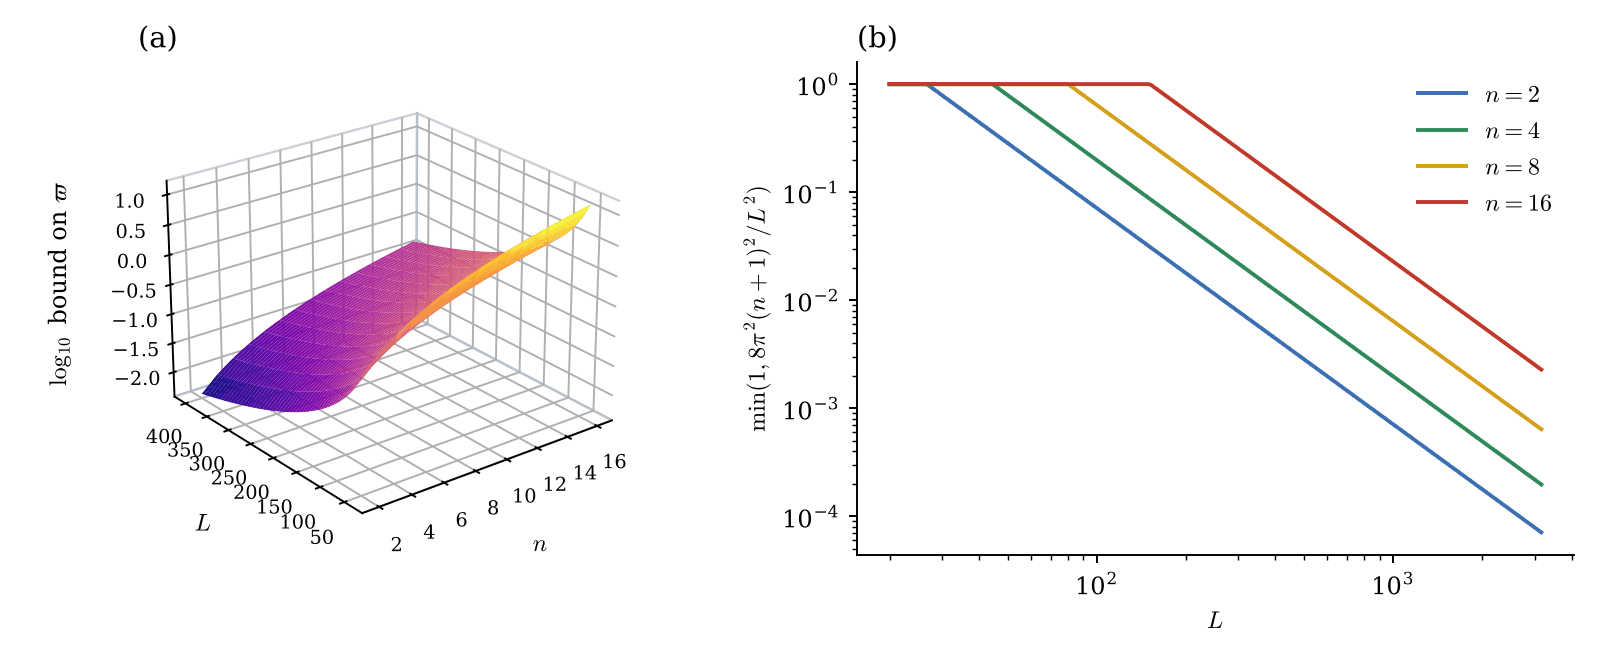
\includegraphics[width=0.92\textwidth]{figures/fig_maxwell.png}
\caption{The Maxwell obstruction (Theorem~\ref{rD:maxwell}). (a) The
logarithm of the bound $8\pi^2(n+1)^2/L^2$ on any constant $\varpi$ of
$\mathrm{BP}(n,\varpi)$ for the Maxwell field, over the cube side $n$ and
the side $L$ of the torus. (b) The bound $\min(1,8\pi^2(n+1)^2/L^2)$ against
$L$ for $n=2,4,8,16$: for every fixed $n$ it tends to $0$ like $L^{-2}$.}
\label{fig:maxwell}
\end{figure*}

\begin{proof}
Let $c\in C^2$ be the cochain with $c_{(y,12)}=\cos(2\pi y_1/L)$ and all
other components zero, so that $f=\ip cF$. The cochain $c$ is exact: with
$g(m)=\sum_{0\le j<m}\cos(2\pi j/L)$, a function on $\Z/L\Z$ because
$\sum_{j=0}^{L-1}\cos(2\pi j/L)=0$, let $A_{(y,2)}=g(y_1)$ and $A_{(y,a)}=0$
for $a\ne2$. Then $(dA)_{(y,12)}=A_{(y,1)}+A_{(y+e_1,2)}-A_{(y+e_2,1)}-
A_{(y,2)}=g(y_1+1)-g(y_1)=c_{(y,12)}$, while $(dA)_{(y,02)}=A_{(y+e_0,2)}-
A_{(y,2)}=0$, $(dA)_{(y,23)}=A_{(y,2)}-A_{(y+e_3,2)}=0$, and the components
in the planes not containing the direction $2$ vanish. Hence $\Pi c=c$ and
$\Var(f)=\beta^{-1}\lVert c\rVert^2=\beta^{-1}L^3\sum_{y_1\in\Z/L\Z}\cos^2
(2\pi y_1/L)=L^4/(2\beta)$, as $L\ge4$.

Fix $x$. Write $c=c^{\rm ext}+c^{\rm in}$ with $c^{\rm in}=c\,1_{P(V_x)}$.
By Lemma~\ref{rD:layer}(i) the support of $c^{\rm in}$ is the disjoint
union of the layers $R_t$ of the plane $\{1,2\}$, $t$ ranging over the
$n^2$ transverse positions. Put $\bar c=\cos(2\pi(x_1-1)/L)$,
$\Phi_t=\sum_{p\in R_t}F_p$ and
\[
g=\ip{c^{\rm ext}}F+\bar c\sum_t\Phi_t .
\]
The variables $F_p$, $p\notin P(V_x)$, are $\mathcal G_x$-measurable by
hypothesis; so is each $\Phi_t$, because $F\in B$ satisfies $dF=0$ and
Lemma~\ref{rD:walls} writes $\Phi_t$ as a linear combination of $F_p$ with
$p\notin P(V_x)$. Hence $g$ is $\mathcal G_x$-measurable, $P_xg=g$, and
since $I-P_x$ is an orthogonal projection,
\[
\begin{split}
\E\lvert f-P_xf\rvert^2&=\E\lvert(I-P_x)(f-g)\rvert^2\le\E\lvert f-g
\rvert^2\\
&=\beta^{-1}\lVert\Pi h\rVert^2\le\beta^{-1}\lVert h\rVert^2,\qquad
h=c^{\rm in}-\bar c\sum_t1_{R_t}.
\end{split}
\]
The cochain $h$ is supported on the $n^2((n+1)^2-1)$ plaquettes of the
layers, and on $(y,12)\in R_t$ its value is $\cos(2\pi y_1/L)-\cos(2\pi
(x_1-1)/L)$ with $y_1=x_1-1+j$, $j\in[0,n]$; since $\cos(2\pi\,\cdot/L)$ is
well defined on $\Z/L\Z$ and $\lvert\cos a-\cos b\rvert\le\lvert a-b\rvert$,
$\lvert h_p\rvert\le2\pi j/L\le2\pi n/L$. Therefore $\lVert h\rVert^2\le
n^2((n+1)^2-1)(2\pi n/L)^2\le4\pi^2n^4(n+1)^2/L^2$, which is the bound for
one cube; summing over the $L^4$ cubes and dividing by $n^4$ gives the
Dirichlet form bound. If $\mathrm{BP}(n,\varpi)$ holds, then $\varpi L^4/
(2\beta)\le4\pi^2(n+1)^2L^2/\beta$, that is $\varpi\le8\pi^2(n+1)^2/L^2$.
\end{proof}

\begin{remark}[what the proof uses, and the exact first-chaos constant]
\label{rD:maxwellremark}
The proof uses two facts only: that $f$ is a slowly varying superposition
of the field strength over one plane, and that the total flux of $F$
through each layer read by a cube is conserved by the move at that cube up
to exterior terms (Lemmas \ref{rD:layer}, \ref{rD:walls}). It does not use
the Gaussian law beyond the identity $\E\ip hF^2=\beta^{-1}\lVert\Pi h
\rVert^2\le\beta^{-1}\lVert h\rVert^2$, and it does not depend on which of
the two natural exterior $\sigma$-algebras is used. For $\mathcal G_x=
\mathcal G_{V_x}$, Lemma~\ref{rD:gaussresp} gives the exact Dirichlet form
of every linear functional, $n^{-4}\sum_x\beta^{-1}\lVert P_{D_{V_x}}c
\rVert^2=\beta^{-1}\ip c{Mc}$ with $M=n^{-4}\sum_xP_{D_{V_x}}$, so that
$\mathrm{BP}(n,\varpi)$ for $\gamma_\beta$ implies $\varpi\le\varpi_1(n,L)$,
the least eigenvalue of $M$ on $B$. The operator $M$ commutes with the
translations of $\Lambda_L$ and is block diagonal in Fourier space with
$6\times6$ blocks, one for each momentum, and $B$ has dimension three in
each block of nonzero momentum. A finite computation of these blocks
gives $\varpi_1(n,L)L^2/(2\pi)^2=0.276$, $0.299$, $0.317$, $0.324$, $0.329$
for $n=2$ and $L=6,8,12,16,24$, and $0.469$, $0.518$, $0.537$, $0.551$ for
$n=3$ and $L=8,12,16,24$, the minimum being attained at the lowest nonzero
momentum (for $L\le8$ all momenta were examined, for $L\ge12$ those with
$\lvert k\rvert_1\le2$); the constant $8\pi^2(n+1)^2$ of the theorem is
$55$ to $70$ times larger than the computed $\varpi_1L^2$. These numbers are
a finite computation and not a proof of any statement about $\varpi_1$
beyond the listed values; the theorem is the proved bound.
\end{remark}

\subsubsection{Two necessary conditions for the averaged estimate}

For a bounded real $O\in\mathcal A$ depending on the links with base points
in $b+[0,s)^4$, and $y\in\Lambda_L$, let $O_y=O\circ\tau_{-y}$ be its
translate, depending on the links with base points in $b+y+[0,s)^4$, and
let $\chi_L(O)=L^{-4}\Var_\mu\bigl(\sum_yO_y\bigr)=\sum_y\Cov_\mu(O_0,O_y)$
be its susceptibility; the last equality uses the translation invariance
of $\mu$ on $\Lambda_L$.

\begin{proposition}[susceptibilities]\label{rD:suscept}
Let $\mathrm{BP}(n,\varpi)$ hold for $\mu$ on $\Lambda_L$, and let $O$ be as
above with $1\le s$ and $n+s\le L$. Then
\[
\chi_L(O)\le\frac{(n+s-1)^8}{n^4\varpi}\Var_\mu(O).
\]
\end{proposition}

\begin{proof}
Put $f=\sum_yO_y$, a real element of $\mathcal A$ with $\Var_\mu(f)=L^4
\chi_L(O)$. For fixed $x$, $(I-\mathcal P_x)O_y=0$ unless a link of the
support of $O_y$ lies in $V_x$, that is unless $x-y-b\in u-v$ for some
$u\in[0,s)^4$, $v\in[0,n)^4$; the set $(-n,s)^4$ of such differences has
$(n+s-1)^4$ elements, which are distinct residues modulo $L$ because
$n+s-1<L$. For each such $y$, $\lVert(I-\mathcal P_x)O_y\rVert_2\le\lVert
O_y-\mu(O_y)\rVert_2=\Var_\mu(O)^{1/2}$, because $I-\mathcal P_x$ is an
orthogonal projection annihilating constants. Hence $\lVert(I-\mathcal P_x)
f\rVert_2\le(n+s-1)^4\Var_\mu(O)^{1/2}$ and $\mathcal E_n(f)\le n^{-4}L^4
(n+s-1)^8\Var_\mu(O)$. The condition $\mathrm{BP}(n,\varpi)$ gives
$\varpi L^4\chi_L(O)\le\mathcal E_n(f)$.
\end{proof}

\begin{corollary}[correlation lengths]\label{rD:xi}
Let $\mathcal L$ be an infinite set of even integers $L\ge2n+4$ such that
$\mathrm{BP}(n,\varpi)$ holds for $\mu_L$ on $\Lambda_L$ for every $L\in
\mathcal L$, and let $\omega$ be a torus limit along $\mathcal L$. Let $f,g$
be bounded local gauge-invariant functions and suppose that there are
$c_0>0$, $\xi>0$ and infinitely many integers $d$ with
\[
\bigl\lvert\omega(f\,\tau_dg)-\omega(f)\omega(g)\bigr\rvert\ge c_0e^{-d/\xi},
\]
where $\tau_d$ is the translation by $d$ lattice units in a fixed
direction. Then
\[
\varpi\le\frac{e^2q_nn}\xi,\qquad\text{equivalently}\qquad\xi\le\frac{e^2q_n
n}\varpi .
\]
In the normalisation of Theorem~\ref{thm:avgtransfer}, $na\le\ell$ and
$\xi=1/(ma)$ with $m$ the physical inverse correlation length, this reads
$\varpi\le e^2q_n\,m\ell$.
\end{corollary}

\begin{proof}
For fixed $d$ and all $L\in\mathcal L$ large enough, $f$ and $\tau_dg$
depend on links of sets $S_f,S_g\subset\Lambda_L$ with $\lvert S_f\rvert,
\lvert S_g\rvert$ independent of $L$ and $d$, at torus distance
$d(S_f,S_g)\ge d-c$ with $c$ depending on $f,g$ only. The second bound of
Theorem~\ref{thm:avgdecay}, which holds for every distance, gives
$\lvert\Cov_{\mu_L}(f,\tau_dg)\rvert\le C(1+d)e^{-\varpi d/(e^2q_nn)}$ with
$C$ independent of $L$ and $d$ (the factor $e^{\varpi c/(e^2q_nn)}\le e^{c}$
is absorbed in $C$, as $\varpi\le4$ and $q_n>16$). The
torus limit is the limit of $\mu_L(f\,\tau_dg)$, $\mu_L(f)$, $\mu_L(g)$
along $\mathcal L$, so $c_0e^{-d/\xi}\le C(1+d)e^{-\varpi d/(e^2q_nn)}$ for
infinitely many $d$. Taking logarithms, dividing by $d$ and letting $d\to
\infty$ along these values gives $-1/\xi\le-\varpi/(e^2q_nn)$.
\end{proof}

\subsubsection{Local functions: the Dirichlet form between two conditional
variances}

\begin{proposition}[local functions]\label{rD:local}
Let $L\ge2n+4$, let $f\in\mathcal A$ be real and depend only on the links
of a set $S$ whose base points lie in a box $b+[0,s)^4$ with $1\le s\le n$.
Then
\[
\begin{split}
\Bigl(\frac{n-s+1}n\Bigr)^4\mu\bigl(\Var_\mu(f\mid\mathcal F_S)\bigr)&\le
\mathcal E_n(f)\\
&\le\Bigl(\frac{n+s-1}n\Bigr)^4\Var_\mu(f).
\end{split}
\]
If $f$ depends only on the four links of a plaquette $p$, then
\[
\Bigl(\frac{n-1}n\Bigr)^2\mu\bigl(\Var_\mu(f\mid\mathcal F_p)\bigr)\le
\mathcal E_n(f)\le\Bigl(1+\frac2n\Bigr)\Var_\mu(f),
\]
where $\mathcal F_p$ is the $\sigma$-algebra of the links not in $p$.
\end{proposition}

\begin{proof}
If $\mathcal G\subset\mathcal F$ are $\sigma$-algebras and $E_{\mathcal G}$,
$E_{\mathcal F}$ the conditional expectations, then $E_{\mathcal G}f=
E_{\mathcal G}E_{\mathcal F}f$ and, by Pythagoras' theorem, $\mu((f-E_{
\mathcal G}f)^2)=\mu((f-E_{\mathcal F}f)^2)+\mu((E_{\mathcal F}f-E_{\mathcal
G}f)^2)\ge\mu((f-E_{\mathcal F}f)^2)=\mu(\Var_\mu(f\mid\mathcal F))$. If
$S\subset V_x$ then $\mathcal F_{V_x}\subset\mathcal F_S$, so $\mu((f-
\mathcal P_xf)^2)\ge\mu(\Var_\mu(f\mid\mathcal F_S))$. The box $b+[0,s)^4$
lies in $x+[0,n)^4$ for exactly $(n-s+1)^4$ values of $x$, which gives the
lower bound. For the upper bound, $(I-\mathcal P_x)f=0$ unless a base point
of $S$ lies in $x+[0,n)^4$, which happens for at most $(n+s-1)^4$ values
of $x$ as in the proof of Proposition~\ref{rD:suscept} ($n+s-1<L$), and
each term is at most $\Var_\mu(f)$. For a plaquette, Lemma~\ref{rD:layer}(i)
gives $n^2(n-1)^2$ cubes containing all four links and $n^2((n+1)^2-1)=
n^4+2n^3$ cubes reading at least one of them.
\end{proof}

\subsubsection{The single-link law of $\SU(2)$ and the plaquette at weak
coupling}

We identify $\SU(2)$ with the unit quaternions $S^3\subset\R^4$, $U=u_0+u_1
\mathbf i+u_2\mathbf j+u_3\mathbf k$, so that $\Tr U=2u_0=2\ip U1$ and
$\Tr(US)=2\operatorname{Re}(US)=2\ip U{\bar S}$, where $\bar S$ is the
conjugate quaternion $S^{-1}$ and $\ip\cdot\cdot$ the Euclidean inner
product of $\R^4$; Haar measure is the normalised surface measure. For a
unit vector $\hat w\in S^3$ and $a>0$ let $\nu_{a,\hat w}$ be the law with
density proportional to $e^{a\ip U{\hat w}}$ with respect to Haar measure.
Writing $U=\cos\theta\,\hat w+\sin\theta\,u$ with $\theta\in[0,\pi]$ and
$u$ in the unit sphere $S^2$ of $\hat w^\perp$, Haar measure is the product
of the density $\frac2\pi\sin^2\theta\,d\theta$ and the uniform law of $u$;
hence under $\nu_{a,\hat w}$ the angle $\theta$ has density proportional to
$e^{a\cos\theta}\sin^2\theta$ on $[0,\pi]$ and $u$ is uniform on $S^2$ and
independent of $\theta$. Expectations under this law are written $\E$.

\begin{lemma}[the single-link law]\label{rD:vmf}
Let $a>0$ and $\hat w\in S^3$.
\begin{enumerate}[label=\textup{(\roman*)},leftmargin=*]
\item For every unit vector $v\in\R^4$ with $\ip v{\hat w}=\cos\alpha$,
\[
\Var_{\nu_{a,\hat w}}\ip Uv=\cos^2\alpha\,\Var(\cos\theta)+\frac{\sin^2
\alpha}3\,\E\sin^2\theta .
\]
\item $a\E\sin^2\theta=3\E\cos\theta$, so that $\E\cos^2\theta=1-3\E\cos
\theta/a$; and $a\E\sin^4\theta=5\E(\sin^2\theta\cos\theta)\ge0$.
\item $\Var(\cos\theta)\ge(\E\cos\theta)^2/a^2$.
\item $\nu_{a,\hat w}(\cos\theta<0)\le3\pi/(2a^2)$, and
\[
\E\cos\theta\ge\frac{1-3\pi/a^2}{1+3/a}.
\]
\item If $a\ge6$, then $\E\cos\theta\ge0.4921$ and $\Var_{\nu_{a,\hat w}}
\ip Uv\ge0.24/a^2$ for every unit vector $v$.
\end{enumerate}
\end{lemma}

\begin{proof}
(i) Write $v=\cos\alpha\,\hat w+\sin\alpha\,v'$ with $v'$ a unit vector of
$\hat w^\perp$ (any one if $\sin\alpha=0$). Then $\ip Uv=\cos\alpha\cos
\theta+\sin\alpha\sin\theta\ip u{v'}$. Since $u$ is uniform on $S^2$ and
independent of $\theta$, $\E\ip u{v'}=0$ and $\E\ip u{v'}^2=\frac13$, so
$\E\ip Uv=\cos\alpha\,\E\cos\theta$ and $\E\ip Uv^2=\cos^2\alpha\,\E\cos^2
\theta+\frac13\sin^2\alpha\,\E\sin^2\theta$, which gives the formula.

(ii) For $k\ge0$,
\[
\begin{split}
\frac d{d\theta}\bigl(e^{a\cos\theta}\sin^{2k+3}\theta\bigr)&=e^{a\cos
\theta}\sin^{2k+2}\theta\\
&\quad\times\bigl((2k+3)\cos\theta-a\sin^2\theta\bigr),
\end{split}
\]
and the left side integrates to zero over $[0,\pi]$. Dividing by
$Z=\int_0^\pi e^{a\cos\theta}\sin^2\theta\,d\theta$ gives $a\E\sin^{2k+2}
\theta=(2k+3)\E(\sin^{2k}\theta\cos\theta)$; $k=0$ and $k=1$ are the first
and third identities, the second is $\E\cos^2\theta=1-\E\sin^2\theta$, and
$\E\sin^4\theta\ge0$ gives the sign.

(iii) Put $S=3\cos\theta-a\sin^2\theta$. For a smooth $g$ on $[0,\pi]$,
\[
\begin{split}
\frac d{d\theta}\bigl(g(\theta)e^{a\cos\theta}\sin^3\theta\bigr)&=e^{a\cos
\theta}\sin^2\theta\\
&\quad\times\bigl(g'(\theta)\sin\theta+g(\theta)S(\theta)\bigr),
\end{split}
\]
so $\E(g'\sin\theta)=-\E(gS)$. With $g=1$, $\E S=0$; with $g=\cos\theta$,
$\E\sin^2\theta=\E(S\cos\theta)=\Cov(\cos\theta,S)$. By the Cauchy--Schwarz
inequality and (ii),
\[
\begin{split}
(\E\sin^2\theta)^2&\le\Var(\cos\theta)\,\E S^2,\\
\E S^2&=9\E\cos^2\theta-6a\E(\sin^2\theta\cos\theta)+a^2\E\sin^4\theta\\
&=9\E\cos^2\theta-a\E(\sin^2\theta\cos\theta)\le9 .
\end{split}
\]
By (ii), $\E\sin^2\theta=3\E\cos\theta/a$, so the left side equals
$9(\E\cos\theta)^2/a^2$; dividing by $9$ gives the claim.

(iv) On $[0,\pi/2]$, $e^{a\cos\theta}\ge1+a\cos\theta$, so $Z\ge\int_0^{\pi
/2}(1+a\cos\theta)\sin^2\theta\,d\theta=\frac\pi4+\frac a3\ge\frac a3$. With
$\theta=\pi/2+\phi$ and $\sin\phi\ge2\phi/\pi$ on $[0,\pi/2]$,
\[
\begin{split}
\int_{\pi/2}^\pi e^{a\cos\theta}\sin^2\theta\,d\theta&=\int_0^{\pi/2}e^{-a
\sin\phi}\cos^2\phi\,d\phi\\
&\le\int_0^{\pi/2}e^{-2a\phi/\pi}d\phi\le\frac\pi{2a},
\end{split}
\]
so $\nu_{a,\hat w}(\cos\theta<0)\le\frac\pi{2a}\cdot\frac3a$. Pointwise
$\cos\theta\ge\cos^2\theta-2\cdot1_{\{\cos\theta<0\}}$, since $\cos\theta
\ge\cos^2\theta$ when $\cos\theta\ge0$ and $\cos\theta\ge-1\ge\cos^2\theta
-2$ always. Taking expectations and using (ii), $\E\cos\theta\ge1-3\E\cos
\theta/a-3\pi/a^2$, which is the second claim.

(v) The bound of (iv) increases with $a$, and at $a=6$ it equals
$(1-\pi/12)/(3/2)\ge0.4921$. By (iii), $\Var(\cos\theta)\ge0.4921^2/a^2\ge
0.24/a^2$; by (ii), $\frac13\E\sin^2\theta=\E\cos\theta/a\ge0.49/a\ge0.24/
a^2$ as $a\ge6$. By (i), $\Var\ip Uv\ge(\cos^2\alpha+\sin^2\alpha)\,0.24/
a^2$.
\end{proof}

\begin{proposition}[the plaquette at weak coupling]\label{rD:plaquette}
Let $G=\SU(2)$ with $\varphi(U)=e^{-2\beta(2-\Tr U)}$, $\beta\ge100$, $n\ge
2$ and $L\ge2n+4$. Let $p$ be a plaquette, $e$ one of its links, and
$\mathcal F_e$ the $\sigma$-algebra of all links other than $e$. Then
\begin{enumerate}[label=\textup{(\roman*)},leftmargin=*]
\item $\mu\bigl(\Var_\mu(\Tr U_p\mid\mathcal F_e)\bigr)\ge1/(1200\beta^2)$;
\item $\Var_\mu(\Tr U_p)\le4(\log\beta+6.11)/\beta$;
\item the Dirichlet form satisfies
\[
\begin{split}
\mathcal E_n(\Tr U_p)&\ge\Bigl(\frac{n-1}n\Bigr)^2\frac1{1200\beta^2}\\
&\ge\Bigl(\frac{n-1}n\Bigr)^2\frac{\Var_\mu(\Tr U_p)}{4800\,\beta(\log
\beta+6.11)}.
\end{split}
\]
\end{enumerate}
In particular the inequality of $\mathrm{BP}(n,\varpi)$ holds for the
functions $\Tr U_p$ with $\varpi=\varpi_p(n,\beta)=((n-1)/n)^2/(4800\beta
(\log\beta+6.11))$, uniformly in $L\ge2n+4$ and in $p$.
\end{proposition}

\begin{proof}
(i) Under $\mu$ the conditional density of $U_e$ given $\mathcal F_e$ is
proportional to $\prod_{p'\ni e}\varphi(U_{p'})$, hence to $\exp(2\beta
\sum_{p'\ni e}\Tr U_{p'})$, the product running over the six plaquettes
containing $e$. For each of them, $U_{p'}$ is a product of four link
variables or their inverses in which $U_e^{\pm1}$ occurs once; by
cyclicity $\Tr U_{p'}=\Tr(U_e^{\pm1}S_{p'})$ with $S_{p'}\in\SU(2)$ the
product of the other three factors in cyclic order, an $\mathcal
F_e$-measurable variable, and since traces on $\SU(2)$ are real and
$\Tr(M^{-1})=\overline{\Tr M}$, $\Tr(U_e^{-1}S)=\Tr(S^{-1}U_e)=\Tr(U_eS^{-1}
)$. Thus $\Tr U_{p'}=\Tr(U_eS'_{p'})=2\ip{U_e}{\bar S'_{p'}}$ with $S'_{p'}
\in\{S_{p'},S_{p'}^{-1}\}$, and the conditional density is proportional to
$\exp(4\beta\ip{U_e}w)$, $w=\sum_{p'\ni e}\bar S'_{p'}\in\R^4$, $\lvert w
\rvert\le6$. In the same way $\Tr U_p=2\ip{U_e}v$ with $v=\bar S'_p$ a unit
vector measurable with respect to $\mathcal F_e$. If $w\ne0$ the conditional
law is $\nu_{a,\hat w}$ with $a=4\beta\lvert w\rvert\le24\beta$ and $\hat w=
w/\lvert w\rvert$, so by Lemma~\ref{rD:vmf}(v), on the event $\{a\ge6\}$,
\[
\begin{split}
\Var_\mu(\Tr U_p\mid\mathcal F_e)&=4\Var_{\nu_{a,\hat w}}\ip Uv\\
&\ge\frac{0.96}{a^2}\ge\frac{0.96}{576\beta^2}=\frac1{600\beta^2}.
\end{split}
\]
On the event $\{a<6\}$ (which contains $\{w=0\}$), $\lvert w\rvert<3/(2
\beta)$ and
\begin{gather*}
\sum_{p'\ni e}\Tr U_{p'}=2\ip{U_e}w\le2\lvert w\rvert<\frac3\beta,\\
\text{so}\qquad\sum_{p'\ni e}(2-\Tr U_{p'})>12-\frac3\beta\ge11.97,
\end{gather*}
and one of the six terms exceeds $1.99$. By Markov's inequality and
Lemma~\ref{lem:bpflat}, which applies as $\beta\ge1$, and by the
equivalence of all plaquettes under the symmetries of $\Lambda_L$,
\[
\begin{split}
\mu(a<6)&\le\sum_{p'\ni e}\mu(2-\Tr U_{p'}>1.99)\\
&\le\frac6{1.99}\cdot\frac{\log\beta+6.11}\beta\le3.02\,\frac{\log\beta+6.11}
\beta\le\frac12,
\end{split}
\]
the last step because $(\log\beta+6.11)/\beta$ decreases on $[1,\infty)$
and equals $0.1072$ at $\beta=100$, where $3.02\cdot0.1072<0.33$. Hence
$\mu(\Var_\mu(\Tr U_p\mid\mathcal F_e))\ge\mu(a\ge6)/(600\beta^2)\ge1/(1200
\beta^2)$.

(ii) Since $0\le2-\Tr U_p\le4$, $\Var_\mu(\Tr U_p)\le\mu((2-\Tr U_p)^2)\le
4\mu(2-\Tr U_p)\le4(\log\beta+6.11)/\beta$ by Lemma~\ref{lem:bpflat}.

(iii) The $\sigma$-algebra $\mathcal F_p$ of the links not in $p$ is
contained in $\mathcal F_e$, so $\mu(\Var_\mu(\Tr U_p\mid\mathcal F_p))\ge
\mu(\Var_\mu(\Tr U_p\mid\mathcal F_e))$ as in the proof of
Proposition~\ref{rD:local}, and that proposition gives $\mathcal E_n(\Tr
U_p)\ge((n-1)/n)^2\mu(\Var_\mu(\Tr U_p\mid\mathcal F_p))$. Combine with (i)
and (ii).
\end{proof}

\begin{remark}[where the factor $\beta\log\beta$ is lost]\label{rD:plaqloss}
The two sides of Proposition~\ref{rD:plaquette}(iii) are of different
orders in $\beta$: the lower bound $((n-1)/n)^2/(1200\beta^2)$ on the
Dirichlet form of $\Tr U_p$ comes from the single-link law, whose variance
in the direction of $v$ is of order $a^{-2}$ with $a\asymp\beta$ when
$\cos\alpha\ne0$, while the variance bound (ii) comes from the first moment
of $2-\Tr U_p$ through the crude inequality $(2-\Tr U_p)^2\le4(2-\Tr U_p)$.
A bound $\mu((2-\Tr U_p)^2)\le C/\beta^2$ for $\beta\ge\beta_0$ would make
$\varpi_p(n,\beta)\ge((n-1)/n)^2/(1200C)$ independent of $\beta$. Such a
bound, with $C=C_L(1+\ell)^2$, is Theorem~\ref{rDtwo:secondmoment},
and Corollary~\ref{rDtwo:bpplaquette} gives $\varpi=1/(1200C_L(1+\ell)^2)$
for $\beta\ge11$, with the factor $((n-1)/n)^2$ removed. For comparison,
Theorem~\ref{thm:bpfixed}(ii) shows that $\mathrm{BP}(n,\varpi)$ itself
fails on $\Lambda_{2n+4}$ unless $\varpi\le38400n^4(\log\beta+6.11)/\beta$,
through test functions built from Polyakov loops; for $\varpi\le\varpi_p(n,
\beta)$ the plaquette traces are not among the functions that violate it,
and (iii) is a statement about those functions only.
\end{remark}

\subsubsection{The compact $\U(1)$ models: what is proved and what is not}

\begin{remark}[status of the abelian consistency check]\label{rD:abelian}
The uniform averaged estimate must fail for a theory without a mass gap,
and the paper records this for the Villain $\U(1)$ model:
Corollary~\ref{cor:avgcoulomb} shows that for $\beta>\beta_0$ no
$\mathrm{BP}(n,\varpi)$ holds for the free-boundary measures of all boxes,
by Theorem~\ref{thm:avgdecay} and the non-summable two-point function of
the field strength of~\cite[Sect.~2]{FS82}. Theorem~\ref{rD:maxwell} adds
the quantitative mechanism in the Gaussian limit of that phase: the flux of
$F$ through the layers read by a cube is conserved by the move up to
exterior terms, so a superposition of the field strength with wavelength
$L$ relaxes at rate at most $8\pi^2(n+1)^2/L^2$, the diffusive rate. Two
parts of the abelian check remain open and are stated here precisely.
\begin{enumerate}[label=\textup{(\alph*)},leftmargin=*]
\item \emph{The torus.} Theorem~\ref{thm:avgtransfer} and
Corollary~\ref{cor:avggap} are formulated for the tori $\Lambda_L$, while
Corollary~\ref{cor:avgcoulomb} concerns free-boundary boxes, because the
state of~\cite{FS82} is the limit of those. The statement that would close
the check is: for the Villain weight and $\beta>\beta_0$, $\mathrm{BP}(n,
\varpi)$ on $\Lambda_L$ implies $\varpi\le C(n,\beta)/L^2$. The proof of
Theorem~\ref{rD:maxwell} does not transfer as it stands: the field
strength $\Psi_p=\varphi_\beta'(\theta_p)/\varphi_\beta(\theta_p)$ of
Proposition~\ref{prop:coulomb} is a nonlinear function of the plaquette
angle, the flux conservation of Lemma~\ref{rD:walls} holds for the compact
variables $U_p=e^{i\theta_p}$, that is for the layer flux modulo $2\pi$,
and the step $\E\lvert f-P_xf\rvert^2\le\E\lvert f-g\rvert^2$ needs an
exterior-measurable $g$ within $O(n/L)$ of $f$ on every layer, which
requires control of the conditional law of the integer part of the layer
flux given the exterior links. This is a statement about the Villain
measure on the torus that is not available in~\cite{FS82} or~\cite{Gut80}.
\item \emph{Wilson's action.} \cite[Sect.~2.11]{FS82} prove the
masslessness of the photon for the Villain form of the action, define the
field strength for Wilson's form as well, state that most of their arguments
extend to a general class of actions, and mark one step of the proof (the
lower bound in their finite-volume estimate) as one that ``does not obviously
extend to Wilson's form'' and would have to be replaced by a direct
argument, which is not given there; the existence proof of the Coulomb
phase in~\cite{Gut80} is for the Villain form as well. No uniform-in-volume
failure of $\mathrm{BP}(n,\varpi)$ is proved here for the Wilson $\U(1)$
action, at any $\beta$.
\end{enumerate}
\end{remark}

\subsubsection{The missing estimate}

\begin{definition}[the uniform averaged estimate along the tuning]
\label{rD:U}
Let $G=\SU(2)$ with the Wilson weight, let $(\beta_k,a_k)$ be the
couplings and lattice spacings of the continuum tuning of
Theorem~\ref{thm:avgtransfer}, with $\beta_k\to\infty$ and $a_k\to0$, and
let $\ell>0$. The estimate $(\mathrm U)$ at the scale $\ell$ is: there are
$\varpi>0$ and integers $n_k\ge2$ with $n_ka_k\le\ell$ such that for every
$k$ and every even $L\ge2n_k+4$ the Wilson measure of $\Lambda_L$ at
$\beta_k$ satisfies $\mathrm{BP}(n_k,\varpi)$. Its local
form $(\mathrm U_{\rm loc})$ is the same statement with
$\mathrm{BP}_{\rm loc}$ of Definition~\ref{def:bploc} in place of
$\mathrm{BP}$.
\end{definition}

\begin{proposition}[what $(\mathrm U)$ gives and what it costs]
\label{rD:Uconsequences}
Suppose $(\mathrm U_{\rm loc})$ holds at the scale $\ell$ with constants
$\varpi,n_k$. Then:
\begin{enumerate}[label=\textup{(\roman*)},leftmargin=*]
\item for every $k$, every torus limit $\omega_k$ along the even $L\ge2n_k
+4$ has a transfer matrix with spectral gap at least $16\varpi/(625e^2n_k)$
in lattice units, hence at least $16\varpi a_k/(625e^2\ell)$ in the units
of $a_k$; and every continuum limit of the $(\omega_k,O_k)$ of
Theorem~\ref{thm:avgtransfer} has a mass gap of at least $16\varpi/(625e^2
\ell)$ if it is nontrivial;
\item for every $k$ and every pair of bounded local gauge-invariant $f,g$:
if $\lvert\omega_k(f\tau_dg)-\omega_k(f)\omega_k(g)\rvert\ge c_0e^{-d/\xi}$
for some $c_0>0$ and infinitely many $d$, then $\xi\le e^2q_{n_k}n_k/
\varpi$;
\item if $(\mathrm U)$ holds, then in addition $n_k^4\ge\varpi\beta_k/
(38400(\log\beta_k+6.11))$ whenever $\beta_k\ge1$, so $n_k\to\infty$, and
the susceptibility bound of Proposition~\ref{rD:suscept} holds with
$(n_k,\varpi)$ on every even $L\ge2n_k+4$ for every $O$ of side $s$ with
$n_k+s\le L$, in particular for every local $O$ in the sense of
Sec.~\ref{ssec:bpweak}.
\end{enumerate}
\end{proposition}

\begin{proof}
(i) is Corollary~\ref{cor:avggap} and Theorem~\ref{thm:avgtransfer} in the
form of Theorem~\ref{thm:bplocal}(iii). (ii) is Corollary~\ref{rD:xi},
whose proof uses only Theorem~\ref{thm:avgdecay} for local $f$, which
Theorem~\ref{thm:bplocal}(ii) provides under $\mathrm{BP}_{\rm loc}$.
(iii) Theorem~\ref{thm:bpfixed}(ii) applies on $\Lambda_{2n_k+4}$, an
admissible torus, and gives $\varpi\le38400n_k^4(\log\beta_k+6.11)/
\beta_k$; Proposition~\ref{rD:suscept} applies to every admissible torus,
and a local $O$ has side $s\le L/2\le L-n_k$.
\end{proof}

\begin{remark}[the exact obstruction]\label{rD:obstruction}
Proposition~\ref{rD:Uconsequences}(i) shows that $(\mathrm U_{\rm loc})$,
hence $(\mathrm U)$, implies the uniform lattice mass gap $m_k\ge16
\varpi a_k/(625e^2\ell)$ along the whole weak-coupling tuning, which
is the open statement that the continuum step is meant to produce. So
$(\mathrm U)$ is at least as strong as its intended consequence, and no
proof of $(\mathrm U)$ can bypass the mass gap. The functions that
Theorem~\ref{rD:maxwell} and Proposition~\ref{rD:suscept} examine are the
slowly varying superpositions of local observables over the whole torus:
for the free Maxwell field their Dirichlet form is at most of order $(n/L)^2$
times their variance (Theorem~\ref{rD:maxwell}; this is proved for that
field only), while $(\mathrm U)$ requires their variance to be bounded by
their Dirichlet form uniformly in $L$. So $(\mathrm U)$ implies that the
susceptibility of every local observable is bounded uniformly in $L$ at the
scale $n$ (Proposition~\ref{rD:suscept}) and that the correlation length of
every torus limit is at most $e^2q_nn/\varpi$ lattice units
(Corollary~\ref{rD:xi}); the converse implications are not proved.

What is available on the other side is of two kinds. First, the sufficient
condition of the paper is the supremum condition $D^0_L(n,\alpha)$ with
$\alpha<1$, which gives $\mathrm{BP}(n,1-\alpha)$ for all $L\ge2n+4$ at
once (Proposition~\ref{prop:avgsup}, Theorem~\ref{thm:bpstrong}(ii)); it
does not depend on $L$, and Corollary~\ref{cor:bpresponse} excludes
$D^0_L(n,\alpha)$ only for $n^4<(1-\alpha)\beta/(38400(\log\beta+6.11))$,
for $\alpha\le\frac12$ only for $n^4<\beta/(76800(\log\beta+6.11))$; the
choice $n_k=\lfloor\ell/a_k\rfloor$ leaves this range as soon as $a_k\le
\ell\bigl(76800(\log\beta_k+6.11)/\beta_k\bigr)^{1/4}/2$, that is for every
tuning in which $a_k$ tends to zero faster than $\beta_k^{-1/4}$. The first
concrete test of $(\mathrm U)$ is therefore whether $D^0_L(n_k,\alpha)$
holds with $\alpha<1$ uniformly in $k$; this is a statement about one cube
of side $n(\beta)$ with arbitrary exterior, with no averaging, and its
analogue for the massless Gaussian field fails
(Proposition~\ref{prop:gauss}(i)). Second, the single-link
bounds of Proposition~\ref{rD:plaquette} give the inequality of
$\mathrm{BP}$ for the plaquette traces uniformly in $L$, but with a
constant independent of $\beta$ (Corollary~\ref{rDtwo:bpplaquette}),
and only for these functions; the
block-spin results of \cite[Sec.~X\,Q]{BBLR26} give $\mathrm{BP}(n,\frac12)$
for the law $\mu^c$ of the block variables of blocks of side $2^k$ at
$\beta_W\le k+2$ on tori of side at most $e^{2^k/(17k)}$
\cite[Corollary~166]{BBLR26}, and their transfer to the Wilson measure
is \cite[Theorem~114]{BBLR26}, whose fibre hypothesis (F),
$\mu'(\Var(f\mid c))\le C_F\Phi(f)$ for all real $f\in\mathcal A'$, is the
estimate on the conditional law of the fine field given the block field
that is not proved; with it, (X) and the almost-orthogonality hypothesis of
that theorem (its hypothesis (D), not the cube estimate (D) of
Sec.~\ref{sec:inputs}), the split inequality would give $\mathrm{BP}$ for
the Wilson measure on the tori covered by the block-spin range, with a
constant depending on $C_F$, $\rho$ and $R$. None of these yields $\mathrm{BP}(n(\beta),\varpi)$ for a class of
$f$ containing the long-wavelength superpositions of
Proposition~\ref{rD:suscept}.

The precise missing lemma is therefore: \emph{for every $k$, $n=n_k\le
\ell/a_k$ and every even $L\ge2n+4$, every local real $f\in\mathcal A$
satisfies $\lVert\mathcal K^t(f-\mu(f))\rVert_2\le(1-\varpi n^4
/L^4)^t\lVert f-\mu(f)\rVert_2$ for all $t\ge0$}, that is
$(\mathrm U_{\rm loc})$, which by Theorem~\ref{thm:bplocal}(iii) suffices
for the continuum step; by Theorem~\ref{thm:bplocal}(iv) its failure
produces a real $h\in\mathcal A_0$ with $\mathcal E_n(h)<\varpi\Var_\mu(h)$
correlated with a local function, and Theorem~\ref{rD:maxwell} exhibits
the shape of such $h$ in the massless case: a plane wave of the field
strength of the longest wavelength. The results proved here bound the
constant of $(\mathrm U)$ from above: by the inverse correlation length of
the torus limits and by the susceptibilities (Corollary~\ref{rD:xi},
Proposition~\ref{rD:suscept}), and, for the free Maxwell field, by
$8\pi^2(n+1)^2/L^2$ (Theorem~\ref{rD:maxwell}); nothing proved here bounds
it from below except for the plaquette traces, and nothing here proves
$(\mathrm U)$, $(\mathrm U_{\rm loc})$, the averaged condition along the
tuning or a mass gap.
\end{remark}
